\section{RNNIP calibratability}

\subsection{Calibration results}

\def\figpath{figures/ftag/DL1r-calibration}

\begin{figure}[htbp]
    \centering
    \subfloat[]{ 
            \includegraphics[width=0.48\linewidth]{\figpath/fig_01}
    } 
     \subfloat[]{ 
            \includegraphics[width=0.48\linewidth]{\figpath/fig_02}
    } 
    \caption{}
    \label{fig:pflow-calib}
\end{figure}

\subsection{Desiderata for a flipped tagger}


\begin{figure}[htbp]
  \centering
 \includegraphics[width=0.5\textwidth]{figures/ftag/fipped-tagger-graphic}
 \caption{Illustration of how the lifetime signage is less likely to be negative for a long lived particle (from Andy Buckley's slides).}
 \label{fig:lifetime-signage}
\end{figure}


\begin{figure}[htbp]
    \centering
    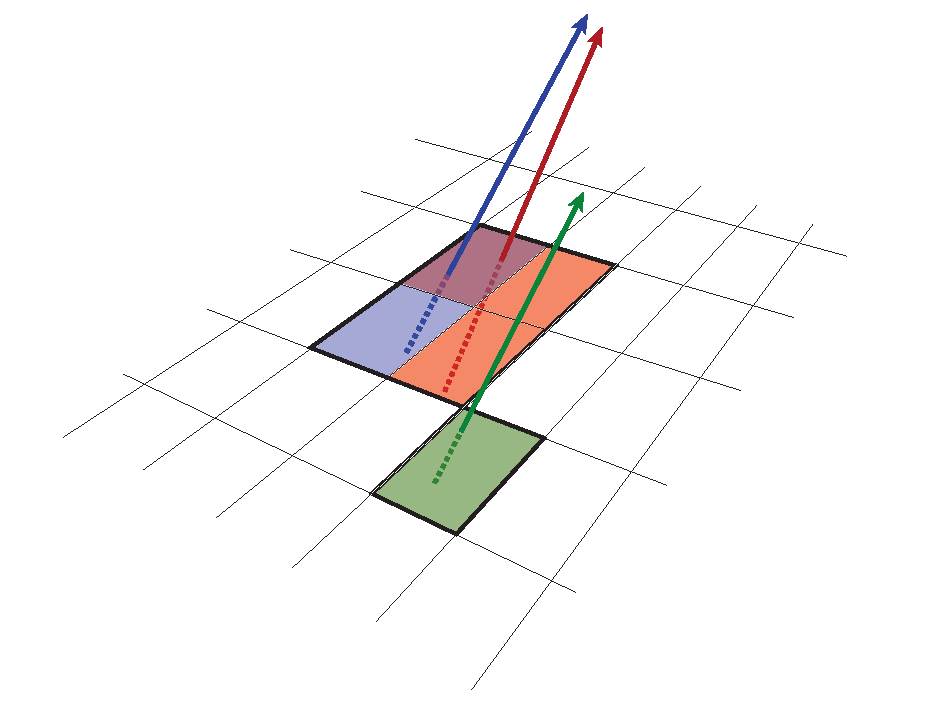
\includegraphics[width=0.8\linewidth]{\figpath/fig_03}
    \caption{}
    \label{fig:pflow-calib-light}
\end{figure}